\chapter{Functional design} \label{chap:func_design}
The functional design presents a high-level overview of the project and what explains what design choices were made on a system-wide level. Additionally, it provides tangential information that can be useful for understanding the working principle of the quantum sensing setup.

%\section{Background knowledge}
%Some background knowledge is required to understand the purpose of the projects, because the setup the project revolves around several non-trivial physics concepts. This section outlines the basic ideas behind the physics that enable the quantum sensing setup to work, from the fundamental physics to how it is used by protocols to measure magnetic field strength.
%
%\subsection{Spin states}
%Spin, at least in quantum mechanics, is the intrinsic angular momentum of a particle,. Importantly, it differs from the angular momentum in classical mechanics, which is extrinsic.
%
%This foundational concept makes it possible to describe quantum systems using various states. The most simple states, used as descriptors, are the energy states. Ground states refer to the system being in an energy minimum. On the other hand, excited states signify that the system has more energy than at its ground state. Additionally, there can be unstable intermediate states during state transition.
%
%While the aforementioned states describe system energy, they have no bearing on the spin. For the purposes of this project, only two spin states need to be explained. The first one is called singlet state. It occurs when an quantum system has a total spin of 0, caused by the mutual cancellation of spin. For example, for a system of two entangled electrons to be a singlet, the two spins directions would need to point in opposite directions. The second spin state is called triplet and it has a total spin of 1. Triplets can consist of, for instance, two unpaired electrons with aligned spins that sum up to 1. Singlets and triplets both have major distinguishing features and properties, which is why they can be used for quantum sensing. Aside from the difference in spin, triplets tend to have higher energy levels. They also exhibit attraction to magnetic fields, while singlets cannot be influenced directly by magnetism.
%
%%\subsection{Energy levels and state transitions} and Zero-field splitting
%\subsection{Zeeman effect}
%Discovered by Pieter Zeeman in 1896, the Zeeman effect is another important phenomenon that enables quantum sensing. If under normal circumstances a light-emitting quantum system emits two spectral lines that almost overlap, then when a magnetic field is applied to it the lines will split, thus exhibiting the Zeeman effect. In an \gls{nv} center, this phenomenon causes the $\ket{\pm1}$ energy level to more clearly split into $\ket{+1}$ and $\ket{-1}$. 
%
%\subsection{Energy levels}\label{chap:energy_levels}
%Figure \ref{fig:energylevels} shows the energy level diagram of an \gls{nv} center.
%\begin{figure}[ht]
%	\centering
%	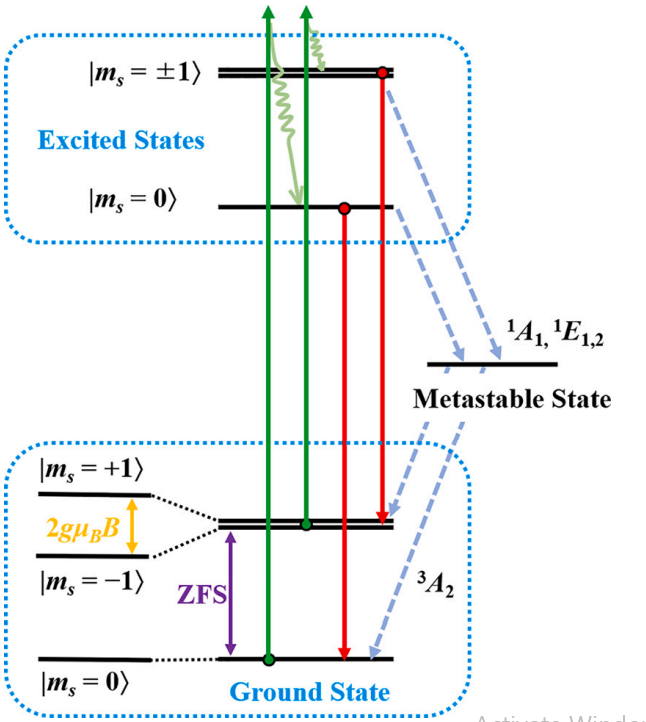
\includegraphics[width=0.7\linewidth]{img/energy_levels}
%	\caption{\gls{nv} center energy level diagram (image credit to Song et al \cite{song2024enhancing})}
%	\label{fig:energylevels}
%\end{figure}
%
%After illuminating the \gls{nv} center with a green laser, electrons go from a ground state to an excited state. They then need to return to the ground state. This decay process is usually direct and emits a red photon, however it can also go through the metastable singlet state and emit an infrared photon. It should be noted that whenever the \gls{nv} center is exposed to the resonant frequency $\nu = 2,87 GHz$ the probability of emitting an infrared photon is significantly increased.


\section{Quantum magnetometry protocols}\label{chap:intro:sequences}
There are a number of different quantum protocols, which differ in what they can measure, in how precisely they can measure it and in the complexity of the hardware they require to operate. \gls{cwodmr} is the main protocol this project is aimed at facilitating. As Saijo et al \cite{saijo2018ac} demonstrate, \gls{cwodmr} is relatively simple, while still detecting magnetic field with reasonable sensitivity. Pulsed protocols outperform \gls{cwodmr} \cite{zhang2020high}, but because of the added complexity working with them requires a more advanced physical setup. Before being able to run other \gls{podmr} on the setup at the lab, three protocols need to be implemented first \cite{sewani2020coherent}. \gls{cwodmr} has already been achieved, but with a different setup and one of the goals of this project is to built towards full \gls{cwodmr}[] support, but with a new and improved setup. $T_1$ measurements, which are one of the fundamentals of \gls{mri}, should be conducted first. Afterwards, Rabi oscillations need to be observed and measured in order to calibrate the setup.



\subsection{\glsfmtshort{cwodmr}}\label{chap:intro:cwodmr}
\gls{cwodmr} is a quantum protocol that has seen extensive usage in sensing setups that measure magnetic fields. Its working principle is centered around the photoluminescence of \gls{nv} centers and the difference in light emission based on spin states.

\begin{figure}[ht]
	\centering
	\begin{tikzpicture}[
		% define box styles
		boxr/.style={rectangle, thick, draw=red!50!black, fill=red!5, minimum size=5mm},
		boxg/.style={rectangle, thick, draw=green!50!black, fill=green!5, minimum size=5mm},
		boxb/.style={rectangle, thick, draw=blue!50!black, fill=blue!5, minimum size=5mm},
		]
		% draw MW nodes
		\node[boxg] (fgen)							{Function generator};
		\node[boxr] (mwsw)		[right=10 mm of fgen] 		{\glsfmtshort{mw} switch};
		\node[boxr] (mwant)		[right=of mwsw]		{\glsfmtshort{mw} antenna};
		\node[boxg] (mwsweep)	[above=of mwsw] 	{Frequency sweeper};
		% draw main system nodes
		\node[boxb] (driver) 	[below=of fgen]		{Current driver};
		\node[boxb] (laser) 	[below=of mwsw]		{Laser};
		\node[boxb] (nv) 		[below=of mwant] 	{NV sample};
		\node[boxb] (detect) 	[right=of nv]		{\textbf{Photodetector}};
		\node[boxg] (daq)		[above=of detect]	{\glsfmtshort{daq}};
		
		
		
		% draw MW lines
		\draw[->, thick] 			(mwsw.east) 		to node[midway, above]{} 	(mwant.west);
		\draw[->, thick]			(mwsweep.south) 	to node[midway, left]{Sweep} 				(mwsw.north);
		% draw main system lines
		\draw[->, thick]			(fgen.south)		to node[midway, left]{Fixed voltage} 					(driver.north);
		\draw[->, thick] 			(driver.east) 		to node[midway, above]{Current} 			(laser.west);
		\draw[->, thick]			(laser.east) 		to node[midway, above]{Light} 				(nv.west);
		\draw[->, thick]			(nv.east) 			to node[midway, above]{Light}				(detect.west);		
		\draw[->, thick]			(detect.north) 		to node[midway, right]{Signal}				(daq.south);	
	\end{tikzpicture}
	\caption{High-level overview of the quantum sensing setup when measuring \gls{cwodmr}[]}
	\label{fig:fd:cwodmr_block}
\end{figure}

Figure \ref{fig:fd:cwodmr_block} shows an overview of the setup for measuring \gls{cwodmr}. A green ($\lambda_{las}$ = 518 \unit[]{\nano\metre}) laser, which emits continuous light, is applied to the crystals, containing the \gls{nv}[] imperfections, and a \gls{mw} generator sweeps through the frequencies\footnote{Typically, the sweep range is from \numrange{2,85}{2,9} \unit{\giga\hertz}. This range might need to be altered in the final version of the sensing setup, but this has no bearing on the photodetector requirements}  near the \gls{nv} center resonant frequency $\nu$ = 2,87 \unit[]{\giga\hertz}. Spin-dependence causes the \gls{nv} center to emit less visible light when exposed to the \gls{mw} signal at the resonant frequency $\nu$. Additionally, two more dips appear on the spectrum if an external magnetic field is applied. After measuring the signal with the photodetector and storing it with the \gls{daq} system, calculating the magnetic field can be done using the formula $h\nu = g_e\mu_BB_{AC}$ \footcite[In the formula, $h$ is the Planck constant, $g_e$ is the g-factor of the electron and $\mu_B$ is the Bohr magneton. Knowing all other variables, $B_{AC}$ can easily be calculated.]{enwiki:1301371272}. 


\begin{figure}[!ht]
	\centering
	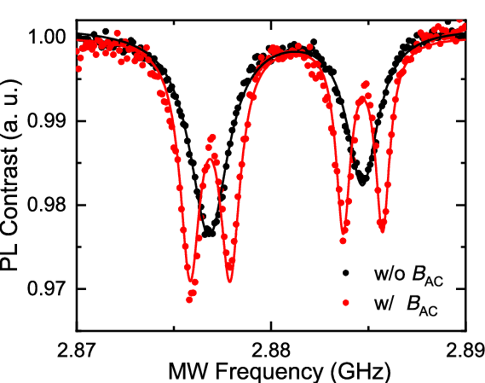
\includegraphics[width=0.7\linewidth]{img/cw_odmr}
	\caption{Example of a \gls{cwodmr} spectrum \textbf{\textcolor{red}{with}} and \textbf{without} a magnetic field present (image credit Saijo et al \cite{saijo2018ac})}
	\label{fig:cwodmr}
\end{figure}

Figure \ref{fig:cwodmr} shows an example of what a \gls{cwodmr} spectrum might look like when a sweep through the near-resonant \gls{mw} frequencies is done. Crucially, the rate of the \gls{mw} frequency sweep has no effect on measurement outcomes. As a result, the sweep causing the \gls{nv} emission changes can be slowed down or sped up based on the bandwidth of the photodetector. \gls{cwodmr} measurements have been carried out with photodetectors with a bandwidth of only 18 \unit[]{\hertz} \cite{acharya2025compact}, which is why the minimum bandwidth for this \gls{cwodmr} photodetector was chosen to be the same.

While the constant light source and \gls{mw} sweep of \gls{cwodmr} lead to a lot of flexibility when designing the photodetector bandwidth, they also make it impossible to use a \gls{lia}. The system simply cannot provide a reference signal to the \gls{lia}, which is required for lock-in amplification. Consequently, a specifically-designed low-noise photodetector \gls{pcb} is needed. After consulting literature \cite{chuprina2026impact}, as well as Applied Nanotechnology expertise, a spectral noise density figure of 5 \unit{\micro\volt\per\hertz\tothe{0.5}} was reached. While the ultimate goal is to keep the total noise under that number, there is an acceptable margin due to limited amount of research on the subject of \gls{cwodmr} photodetector noise.

\begin{table}[!ht]
	\centering
	\begin{tabular}{|c|c|}
		\hline
		Bandwidth 	&  $\geq$ 18 \unit[]{\hertz}					\\
		\hline
		Noise	 	&  $\leq$ 5 \unit{\micro\volt\per\hertz\tothe{0.5}}	\\
		\hline
	\end{tabular}
	\caption{Minimum photodetector requirements for detecting \gls{cwodmr}}
	\label{tab:fd:cwodmr}
\end{table}


\subsection{$T_1$ relaxometry}\label{chap:fd:t1}
\begin{figure}[!ht]
	\centering
	\begin{tikzpicture}[
		% define box styles
		boxr/.style={rectangle, thick, draw=red!50!black, fill=red!5, minimum size=5mm},
		boxg/.style={rectangle, thick, draw=green!50!black, fill=green!5, minimum size=5mm},
		boxb/.style={rectangle, thick, draw=blue!50!black, fill=blue!5, minimum size=5mm},
		]
		
		% boxes
		\node[boxg] (fgen)							{Function generator};
		\node[boxb] (driver) 	[below=of fgen]		{Current driver};
		\node[boxb] (laser) 	[below=of mwsw]		{Laser};
		\node[boxb] (nv) 		[below=of mwant] 	{NV sample};
		\node[boxb] (detect) 	[right=of nv]		{\textbf{Photodetector}};
		\node[boxg] (daq)		[above=of detect]	{\glsfmtshort{daq}};
		
		
		
		% draw main system lines
		\draw[->, thick]			(fgen.south)		to node[midway, left]{\glsfmtshort{ttl}}	(driver.north);
		\draw[->, thick]			(fgen.east)			to node[midway, above]{Reference signal} 	(daq.west);
		\draw[->, thick] 			(driver.east) 		to node[midway, above]{Current} 			(laser.west);
		\draw[->, thick]			(laser.east) 		to node[midway, above]{Light} 				(nv.west);
		\draw[->, thick]			(nv.east) 			to node[midway, above]{Light}				(detect.west);		
		\draw[->, thick]			(detect.north) 		to node[midway, right]{Signal}				(daq.south);	
	\end{tikzpicture}
	\caption{High-level overview of the quantum sensing setup when measuring $T_1$ relaxation time}
	\label{fig:fd:t1_block}
\end{figure}

$T_1$, $T_2$ and $T_2^*$ relaxation time measurements are commonly associated with radiometry \cite{ballinger23}, but they have other uses too. $T_1$ measurements, in particular, are useful in the realm of quantum sensing. Knowing the $T_1$ relaxation time, which refers to the time it takes for the spins in an \gls{nv} system to decay back to their original state, makes it possible to adjust the pulse sequences of the Rabi oscillations protocol and thus get better results. 

Implementing this protocol is more involved than implementing \gls{cwodmr}, even though the setup in Figure \ref{fig:fd:t1_block} is much simpler than the \gls{cwodmr}[] setup in Figure \ref{fig:fd:cwodmr_block}. A specific pulsing sequence needs to be output to drive the laser and altered slightly for every data point that needs to be measured, while the same reference signal is output to the \gls{daq} system throughout the whole experiment. Although the optical data path remains the same, $T_1$ data acquisition is done using a \gls{lia}, whereas \gls{cwodmr} is not. 

\begin{figure}[ht]
	\centering
	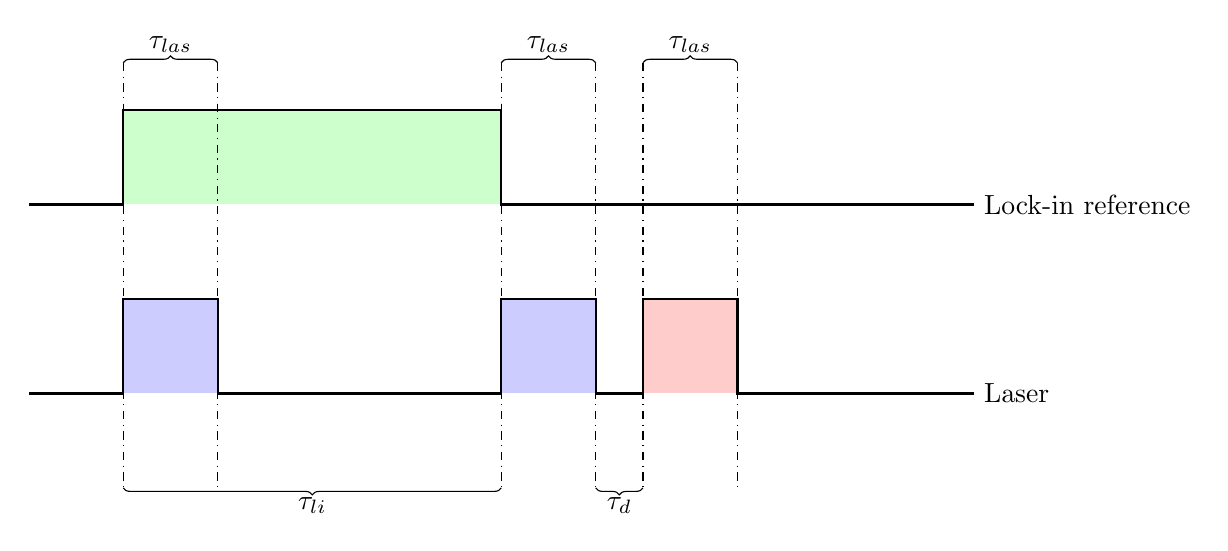
\begin{tikzpicture}[scale=.3]
		% TTL signal rectangles
		\fill [blue!20] 		(4,0) 	rectangle (8,4);
		\fill [blue!20] 		(20,0) 	rectangle (24,4);
		\fill [red!20]			(26,0)	rectangle (30,4);
		\fill [green!20] 		(4,8) 	rectangle (20,12);
		
		% signal lines
		\draw [thick] (0,0) -- (4, 0) -- (4,4) --(8,4) -- (8,0) -- (20,0) -- (20,4) -- (24,4) --(24,0) -- (26,0) -- (26,4) -- (30,4) -- (30,0) -- (40,0) node[anchor=west]{Laser};
		\draw [thick] (0,8) -- (4,8) -- (4,12) -- (20,12) -- (20,8) -- (40,8) node[anchor=west]{Lock-in reference}; % ref
		
		% curly braces top
		\draw [decorate, decoration={brace}] (4,14) -- (8,14) node[midway, above]{$\tau_{las}$};
		\draw [decorate, decoration={brace}] (20,14) -- (24,14) node[midway, above]{$\tau_{las}$};
		\draw [decorate, decoration={brace}] (26,14) -- (30,14) node[midway, above]{$\tau_{las}$};
		
		% curly braces bottom
		\draw [decorate, decoration={brace, mirror}] (4,-4) -- (20,-4) node[midway, below]{$\tau_{li}$};
		\draw [decorate, decoration={brace, mirror}] (24,-4) -- (26,-4) node[midway, below]{$\tau_{d}$};
		
		% dash-dotted lines
		\draw [dash dot] (4,14) -- (4,-4);
		\draw [dash dot] (8,14) -- (8,-4);
		\draw [dash dot] (20,14) -- (20,-4);
		\draw [dash dot] (24,14) -- (24,-4);
		\draw [dash dot] (26,14) -- (26,-4);
		\draw [dash dot] (30,14) -- (30,-4);
		
	\end{tikzpicture}
	\caption{Laser and reference signals for $T_1$ measurements}
	\label{fig:t1waveforms}
\end{figure}


\begin{figure}[!ht]
	\centering
	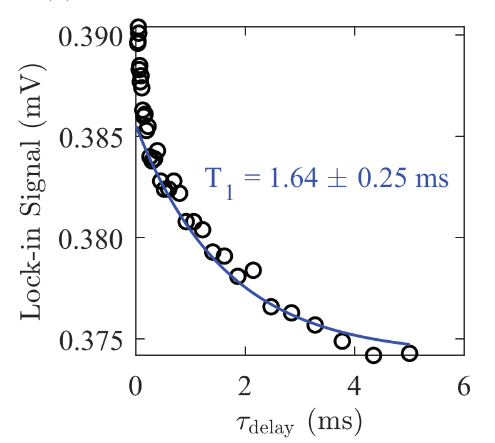
\includegraphics[width=0.5\linewidth]{img/t1_result}
	\caption{Results of a set of $T_1$ measurements with varied dark time $\tau_d$ (image credit to Sewani et al \cite{sewani2020coherent})}
	\label{fig:t1result}
\end{figure}

The waveforms which are needed for $T_1$ measurements are shown if Figure \ref{fig:t1waveforms}. While both are important in practice, the periodic lock-in reference pulse is not as relevant, at least in this section of the report. However, its working principle is explored in Chapter \ref{chap:lockin}. For now, all that needs to be said about the lock-in reference signal is that it is periodic and $\tau_{li}$ is much longer than $\tau_{las}$ (Sewani et al \cite{sewani2020coherent} propose $\tau_{li} = 15 ms$ and $\tau_{las} = 5 \mu s$). Laser pulses, on the other hand, are not simply periodic pulses. Instead, there are three short pulses every reference period (which is $2\tau_{li} s$ long). The two blue pulses have the same timing every cycle, because they initialize the \gls{nv} spins. However, the red pulse always occurs after the variable dark time $\tau_d$, which is increased for every data point. Depending on the $T_1$ decay at the time of the readout pulse, a different amount of light will be emitted by the \gls{nv}[] centers and consequently a different voltage will be detected. Figure \ref{fig:t1result} shows what results can be expected when measuring $T_1$ and varying the dark time. Determining the value of $T_1$ is done using Formula \ref{eq:t1}, where $I$ is the light intensity, $I_\infty$ is the light intensity offset and $\tau_d$ is the dark time. 

\begin{equation}\label{eq:t1}
I(t)=I_\infty+I(0)e^{-\tau_d/T_1}
\end{equation}


When it comes to photodetection, the most important difference between \gls{cwodmr} and $T_1$ measurements is the $T_1$ laser pulsing (see \textbf{Function generator} output in Figures \ref{fig:fd:cwodmr_block} and \ref{fig:fd:t1_block}). Furthermore, utilization of a \gls{lia} changes the noise requirements significantly. This introduces the need for a different photodetector specifically for \gls{podmr}, which trades low-noise signal output for a broad-bandwidth optical pulse detection. In order to develop more specific \gls{podmr} photodetection requirements, they are only discussed after the introduction of the Rabi oscillations protocol in Chapter \ref{chap:fd:podmr}.


\subsection{Rabi oscillations}\label{chap:fd:podmr}
There are several protocols which fall under the \gls{podmr} umbrella. Aside from $T_1$ measurements, Ramsey interferometry, Hahn echo and Rabi oscillations are the most common pulsed protocols. Supporting Rabi oscillations is an important quantum computing milestone for the Applied Nanotechnology research group. For the time being, it is the most important \gls{podmr} protocol, while other pulsed protocols will probably be implemented later on. However, $T_1$ measurements need to be supported first, as based on them the quantum sensing setup will be optimized to detect Rabi oscillations.


\begin{figure}[!ht]
	\centering
	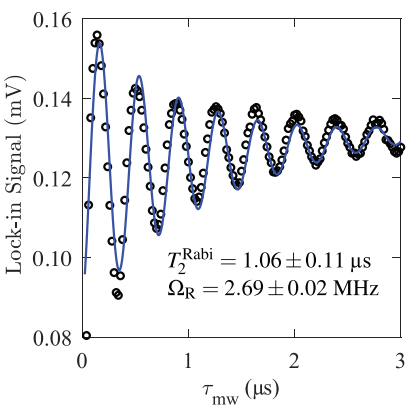
\includegraphics[width=0.5\linewidth]{img/rabi_result}
	\caption{Rabi oscillations measurement (image credit to Sewani et al \cite{sewani2020coherent})}
	\label{fig:fd:rabiresult}
\end{figure}

Rabi oscillations are, as the name suggests, oscillations arising from the variations of the quantum state of the system, which in the case of \gls{nv} centers manifest in a sinusoidal light signal. However, the oscillations of an \gls{nv} system decay over time due to quantum decoherence. The oscillation frequency $\Omega_R$ is called Rabi frequency. Figure \ref{fig:fd:rabiresult} shows what Rabi oscillations look like when measured with an optical setup.

\begin{figure}[!ht]
	\centering
	\begin{tikzpicture}[
		% define box styles
		boxr/.style={rectangle, thick, draw=red!50!black, fill=red!5, minimum size=5mm},
		boxg/.style={rectangle, thick, draw=green!50!black, fill=green!5, minimum size=5mm},
		boxb/.style={rectangle, thick, draw=blue!50!black, fill=blue!5, minimum size=5mm},
		]
		% draw MW nodes
		\node[boxg] (fgen)							{Function generator};
		\node[boxr] (mwsw)		[right=10 mm of fgen] 		{\glsfmtshort{mw} switch};
		\node[boxr] (mwant)		[right=of mwsw]		{\glsfmtshort{mw} antenna};
		% draw main system nodes
		\node[boxb] (driver) 	[below=of fgen]		{Current driver};
		\node[boxb] (laser) 	[below=of mwsw]		{Laser};
		\node[boxb] (nv) 		[below=of mwant] 	{NV sample};
		\node[boxb] (detect) 	[right=of nv]		{\textbf{Photodetector}};
		\node[boxg] (lockin)	[above=of detect]	{\glsfmtshort{daq}};
		
		
		% draw MW lines
		\draw[->, thick] 			(fgen.east) 		to node[midway, above]{\glsfmtshort{ttl}} 	(mwsw.west);
		\draw[->, thick] 			(mwsw.east) 		to node[midway, above]{\glsfmtshort{ttl}} 	(mwant.west);
		% draw main system lines
		\draw[->, thick]			(fgen.south)		to node[midway, left]{\glsfmtshort{ttl}} 	(driver.north);
		\draw[->, thick] 			(driver.east) 		to node[midway, above]{Current} 			(laser.west);
		\draw[->, thick]			(laser.east) 		to node[midway, above]{Light} 				(nv.west);
		\draw[->, thick]			(nv.east) 			to node[midway, above]{Light}				(detect.west);		
		\draw[->, thick]			(detect.north) 		to node[midway, right]{Signal}				(lockin.south);	
		% draw long line
		\draw[->, thick] (fgen.south east) .. controls +(down:5mm) .. node[pos=.9, sloped, below]{Reference signal}(lockin.south west);
	\end{tikzpicture}
	\caption{High-level overview of the quantum sensing setup when measuring Rabi oscillations}
	\label{fig:fd:rabi_block}
\end{figure}

Figure \ref{fig:fd:rabi_block} shows the quantum sensing subsystems which are used during Rabi oscillations experiments. Compared to the $T_1$ measurements setup seen in Figure \ref{fig:fd:t1_block}, the Rabi system is similar, but also makes use of the \gls{mw}[] subsystem. Unlike \gls{cwodmr} experiments, the \gls{mw} signal needs to be pulsed instead of swept. The addition of \gls{mw} pulsing complicates waveform generation, as the \gls{mw}[] pulses need to be programmed in addition to the laser pulses and \gls{daq}[] reference signal.

Figure \ref{fig:fd:rabiwaveforms} shows the pulsing sequences needed to achieve Rabi oscillations. Even though they resemble the $T_1$ sequences somewhat, the Rabi oscillations setup is more convoluted. At the very least, to achieve Rabi oscillations in the \gls{nv}[] centers, a microwave signal is needed, which adds an additional pulse sequence. The microwave pulse width $\tau_{mw}$ is varied, which provides the data points seen in Figure \ref{fig:fd:rabiresult}. Another major difference is that the two halves of the sequences are repeated a number of times.

\begin{figure}[!ht]
	\centering
	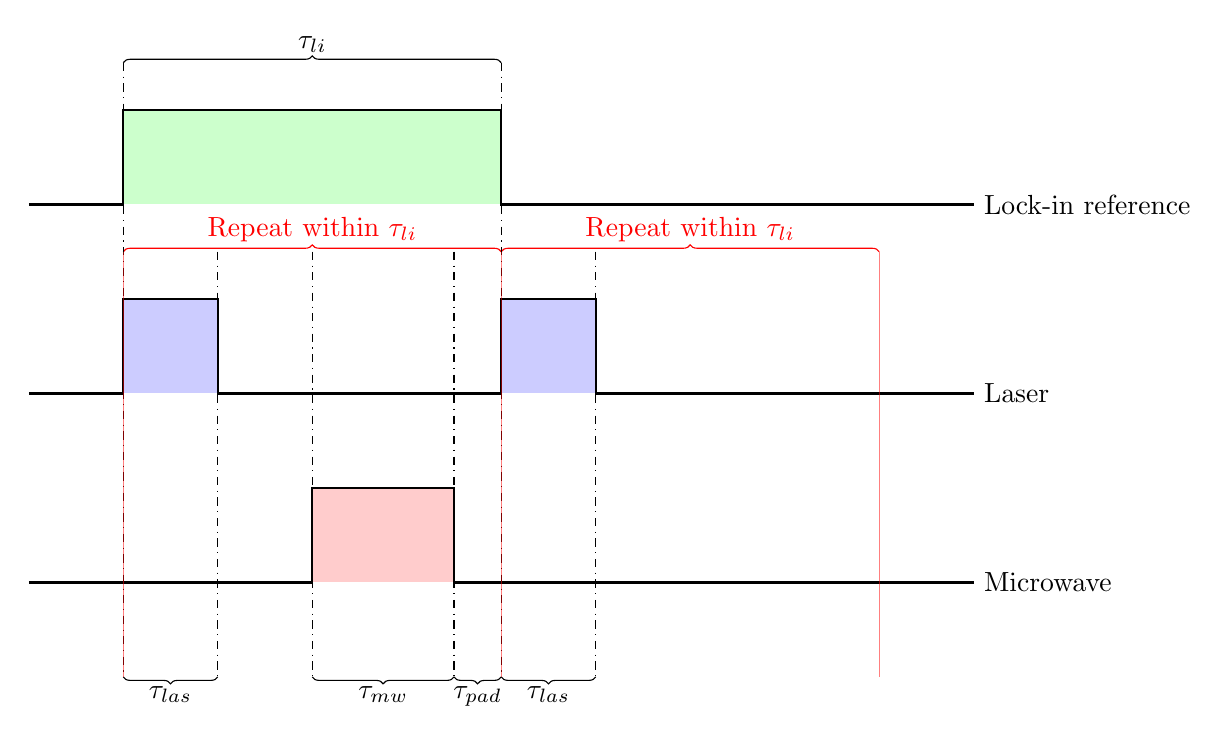
\begin{tikzpicture}[scale=.3]
		% TTL signal rectangles
		\fill [blue!20] 		(4,0) 		rectangle (8,4);
		\fill [blue!20] 		(20,0) 		rectangle (24,4);
		\fill [green!20] 		(4,8) 		rectangle (20,12);
		\fill [red!20]			(12,-8)		rectangle (18,-4);
		
		% signal lines
		\draw [thick] (0,0) -- (4, 0) -- (4,4) --(8,4) -- (8,0) -- (20,0) -- (20,4) -- (24,4) --(24,0) -- (40,0) node[anchor=west]{Laser};
		\draw [thick] (0,8) -- (4,8) -- (4,12) -- (20,12) -- (20,8) -- (40,8) node[anchor=west]{Lock-in reference}; % ref
		\draw [thick] (0, -8) -- (12, -8) -- (12, -4) -- (18, -4) -- (18, -8) -- (40, -8) node[anchor=west]{Microwave}; % mw signal
		
		% curly brace top
		\draw [decorate, decoration={brace}] (4,14)  -- (20,14) node[midway, above]{$\tau_{li}$};
		
		
		% curly braces mid
		\draw [red, decorate, decoration={brace}] (4,6)  -- (20,6) node[midway, above]{Repeat within $\tau_{li}$};
		\draw [red, decorate, decoration={brace}] (20,6) -- (36,6) node[midway, above]{Repeat within $\tau_{li}$};
		

		
		% curly braces bottom
		\draw [decorate, decoration={brace, mirror}] (12,-12) -- (18,-12) node[midway, below]{$\tau_{mw}$};
		\draw [decorate, decoration={brace, mirror}] (18,-12) -- (20,-12) node[midway, below]{$\tau_{pad}$};
		\draw [decorate, decoration={brace, mirror}] (20,-12) -- (24,-12) node[midway, below]{$\tau_{las}$};
		\draw [decorate, decoration={brace, mirror}] (4,-12)  -- (8,-12) node[midway, below]{$\tau_{las}$};
		
		
		% dash-dotted lines
		\draw [dash dot] (4,14)  -- (4,-12);
		\draw [dash dot] (8,6)   -- (8,-12);
		\draw [dash dot] (12,6)  -- (12,-12);
		\draw [dash dot] (18,6)  -- (18,-12);
		\draw [dash dot] (20,14) -- (20,-12);
		\draw [dash dot] (24,6)  -- (24,-12);
		
		% transparent lines
		\draw [red, opacity=0.5] (4,6)  -- (4,-12);
		\draw [red, opacity=0.5] (20,6) -- (20,-12);
		\draw [red, opacity=0.5] (36,6) -- (36,-12);

		
	\end{tikzpicture}
	\caption{Laser and reference signals for the Rabi oscillations protocol}
	\label{fig:fd:rabiwaveforms}
\end{figure}

That being said, $T_1$ measurements and Rabi oscillations are similar enough to where they can share the same photodetector. Both use a \gls{lia} to increase the output \gls{snr} and, as a consequence, do not have the restrictive noise requirements of the \gls{cwodmr} photodetector (see Table \ref{tab:fd:cwodmr}). Due to the addition of another variable factor, namely the \gls{lia}, an exact figure for the noise could not be computed. 

The optical pulses that differentiate \gls{podmr} from \gls{cwodmr} create a need for a photodetector with a much broader bandwidth. To detect the optical signal during $T_1$ measurements, a bandwidth of \numrange[]{1}{2} \unit{\mega\hertz} is needed. However, $T_1$ measurements is less demanding than Rabi oscillations, which needs a photodetector bandwidth of around \numrange[]{3}{4} \unit{\mega\hertz}.  However, based on setups by Sewani et al. \cite{sewani2020coherent}, Nandi et al. \cite{nandi2024oscilloscope} and Murzakhanov et al. \cite{murzakhanov2025mechanism} it was decided the signal bandwidth of the device should be increased to least 5 \unit{\mega\hertz} to create a safety margin. By relegating the noise as a requirement, the \gls{lia} makes the necessary bandwidth increase possible. 

\begin{table}[!ht]
	\centering
	\begin{tabular}{|c|c|}
		\hline
		Bandwidth 	&  $\geq$ 5 \unit[]{\mega\hertz}					\\
		\hline
	\end{tabular}
	\caption{Minimum photodetector requirements for detecting \gls{cwodmr}}
	\label{tab:fd:podmr}
\end{table}




\section{Photodetection}
%Photodetection is how the \gls{nv} photoluminescence is measured, effectively turning light into current using a photodiode. However, a bare photodiode cannot be used as a readout device or connected to a \gls{lia}, because it functions as a current generator. This is where the photodetection \gls {pcb} comes in. Its purpose is to transform the current into voltage and then amplify the resulting signal to the necessary voltage level using a \gls{tia}.
Enabling photodetection specifically for quantum sensing is the main goal of the project. Chapter \ref{chap:intro:sequences} covered the requirements resulting from the physics behind different quantum magnetometry protocols, which are prerequisites for the high-level design discussed in this part of the report. 

\begin{table}[!ht]
	\centering
	\begin{tabular}{|c||c|c|c|}
		\hline
		Subsystem 		& Solution 1 & Solution 2	& Solution 3 \\
		\hline
		Photodetector 	& p-i-n photodiode 	& Avalanche photodiode	& Balanced p-i-n  \\
		\hline
		
		Photodiode biasing 	& Photoconductive	& Photovoltaic	& Bootstrapped 	\\
		\hline
		
		Amplification 	& \gls{tia} only	& \gls{tia} with post-amplifier	 & - \\
		\hline
		
		\gls{tia} 		& Transistor \gls{tia}	& Op-amp \gls{ic} & - \\
		\hline
		
		Post-amplifier 	& Inverting 			& Non-inverting			& Non-standard  	\\
		\hline
		
		System power	& External & Internal	& Hybrid \\
		\hline
		
%		\gls{daq} 		& \gls{ad2} with \gls{lia} & \gls{ad2} without\gls{lia}	& Only \gls{lia} \\
%		\hline
	\end{tabular}
	\caption{List of photodetector subsystems and their possible implementations}
	\label{tab:fd:reqs}
\end{table} 

Table \ref{tab:fd:reqs} lists the main solutions that were considered during the high-level design stage of the V-Model in Figure \ref{fig:vmodel}.

The first consideration when designing a photodetector is what photodetection element will be used for the conversion of optical to electrical signals. While avalanche photodiodes are generally the best option in terms of detection capabilities, their price eliminated them from the discussion early on in the design process, as a single one usually costs two times more than the photodetection \gls{pcb} budget. For that reason, p-i-n photodiodes were selected as an affordable alternative for both \gls{cwodmr} and \gls{podmr} detection, that has also found use in a number of custom quantum sensing photodetectors. Making a photodetection \gls{pcb} with a balanced p-i-n photodetector was also considered. Balancing a photodetector means connecting two photodiodes with a single differential amplifier in order to reduce variability in the signal. Ultimately, it was decided that even if a single diode performs worse on paper, it is still preferred. This choice was made mainly, because balancing the photodetector will increase the optical data path complexity, which is something the client said was not desirable.

After choosing the photodetection device, its biasing should also be discussed. The two most common biasing configurations are photoconductive and photovoltaic. Photoconductive biasing results in a bigger output current, but generates more photodetector noise, while photovoltaic biasing is more low-noise with the disadvantage of outputting lower current. Chapter \ref{chap:fd:photodiodes} covers both in more detail. When designing a \gls{cwodmr} photodetector specifically for low noise, photovoltaic mode is better and hence why it was chosen. However, \gls{podmr} designs need a significantly broader bandwidth and biasing can be used to achieve it. Because noise is less important for this device, bootstrapping became a possibility. Bootstrapped photodetectors have specific biasing circuitry to achieve a broader bandwidth. The concept is explained in greater detail in Chapter \ref{chap:td:v4_design}. Because the bootstrapped photodetector \gls{pcb} had biasing issues when tested (see Chapter \ref{chap:test:v4_results}), an alternative design was proposed. It retains the possibility of biasing the photodetector in photovoltaic mode, while offering the option to bias it in photoconductive mode as well.

The third important design choice that needs to be discussed is the amplification. and its high-level implementation. A \gls{tia} needs to be used to amplify the photodiode current and output it as voltage. Similar photodetection \glspl{pcb} often have a post amplifier. The term refers to any amplifier that is used in conjunction with a \gls{tia} in order to boost its output. The chief benefit of using post amplification is that the input current can be boosted to higher levels without sacrificing bandwidth. However, this comes at the cost of increased output noise. Post amplification was added to the \gls{podmr} \gls{tia} for the increased bandwidth, but the first \gls{cwodmr} iterations also have post amplification. This was done to keep the designs as similar as possible at first, but later it was decided that post amplification contributes too much noise to the system and the final \gls{cwodmr} circuit does not have a post amplifier.

When discussing amplification it is also important to discuss some more specific implementation details. Perhaps the most significant consideration is the device type used to implement the \gls{tia}. \glspl{tia} commonly use either op-amps or transistors. Op-amp \glspl{ic} offer a simpler solution, while transistor \glspl{ic} can give more freedom to adjust the circuit specifications. The drawback of transistors in general is the added complexity when designing and troubleshooting the photodetectors. Transistor \glspl{ic} have an additional disadvantage, because they are prefabricated and thus can be altered less than transistors designed specifically for the circuit. Op-amps photodetectors are certainly less customizable, but the simplicity when working with their theoretical models, as well as the aforementioned drawbacks of transistor designs, was why the designs for both photodetector types use op-amps.

The last amplifier consideration that needs to be discussed is the post-amplifier type. Using an inverting amplifier is an option \cite{acharya2025compact}, however the non-inverting layout was chosen for the \gls{podmr} detector and some of the preliminary \gls{cwodmr} designs. The main reasons for the choice are the increased \gls{cmrr} and input impedance the non-inverting system, as well as the fact that it does not invert the phase of the signal. Another option which was considered for a time was using modified versions of the aforementioned post-amplifier types, like the one proposed by Noh \cite{noh2020frequency}, however due to the added theoretical complexity and limited literature, eventually it was decided that exploring non-standard circuits would be too big of a time investment for the purposes of the project.


The system power circuitry should also be discussed. Using external power (e.g. from a bench power supply) entirely is useful for preliminary designs, owing to the simplified testing and troubleshooting. Additionally, the use of fewer components results in less noise. In comparison, an internal power supply (e.g. from a battery) would contribute more noise, but it would also make the design portable. Portability is not the biggest priority right now. Still, the Applied Nanotechnology research group would like to develop a portable \gls{cwodmr} demonstrator after the lab setup is finished, so a design made with portability in mind will be a good addition to the setup. Hybrid power supply, in this case, refers to the using of an external power supply together with the power circuitry (e.g. voltage converters) of an internal power supply. At first glance, this solution seems redundant, as it combines the disadvantages of both of the previous power supply schemes with seemingly no benefit. This is not the case, as this method of supplying power allows the system to draw power from an unreliable source (e.g. microcontroller) while still supplying constant power to the circuit. This method is simpler and more modular than having an onboard power source. Additionally, it retains much of the portability of an internal power supply system. Because of this, the \gls{cwodmr} design has external and hybrid power supply versions. The \gls{podmr} photodetector does not need an internal or hybrid supply for now, even though in the far future Applied Nanotechnology might make a \gls{podmr} demonstrator as well, which  is why this photodetector uses an external power supply.

%todo: add daq
%Data acquisition is also an important functionality to consider, especially because it is one of the focus points of the software part of this project. 

\subsection{Photodiodes}\label{chap:fd:photodiodes}
At the heart of the photodetector lies the photodiode. It is what turns light into current and the \gls{tia} that follows it only amplifies and translates that current signal to voltage. The specifications of the diode are an important part of the photodetector circuit. Photodiode biasing is another vital aspect of the photodetector, as it dictates the noise levels and bandwidth, thus directly influencing the amplifier design.

\begin{figure}[ht]
	\centering
	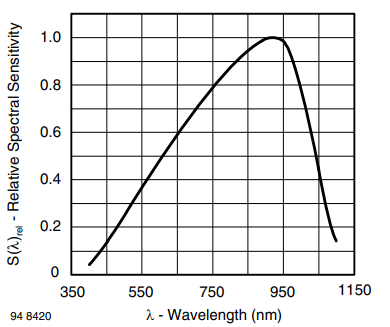
\includegraphics[width=0.5\linewidth]{img/bpw34_sens}
	\caption{BPW34 sensitivity (image credit to the BPW34 documentation \cite{vishay2011bpw34})}
	\label{fig:fd:bpw34sens}
\end{figure}



\begin{figure}[ht]
	\centering
	\begin{subfigure}[1a]{.49\linewidth}
		\begin{circuitikz}
			\tikzstyle{every node}=[font=\normalsize]
			\draw [ line width=0.5pt](3.75,9) to[empty photodiode,l={ \normalsize $D_1$}] (3.75,10.75);
			\draw [ line width=0.5pt](6.5,10.25) node[op amp,scale=1] (opamp2) {};
			\draw [ line width=0.5pt](opamp2.+) to[short] (5,9.75);
			\draw [ line width=0.5pt] (opamp2.-) to[short] (5,10.75);
			\draw [ line width=0.5pt](7.7,10.25) to[short](8,10.25);
			\draw [line width=0.5pt](5,9) to (5,8.25) node[ground]{};
			\draw [ line width=0.5pt](5,8.5) to[short] (5,9.75);
			\draw [ line width=0.5pt](3.75,10.5) to[short] (3.75,10.75);
			\draw [ line width=0.5pt](3.75,10.75) to[short] (5,10.75);
			\node at (4.5,10.75) [circ] {};
			\draw [ line width=0.5pt](4.5,10.75) to[short] (4.5,13.5);
			\draw [ line width=0.5pt](4.5,12.25) to[short] (5,12.25);
			\draw [ line width=0.5pt](4.5,13.5) to[short] (5,13.5);
			\draw [ line width=0.5pt](7.5,10.25) to[short] (7.5,11);
			\draw [ line width=0.5pt](5,12.25) to[european resistor,l={ \normalsize $R_1$}] (7,12.25);
			\node at (4.5,12.25) [circ] {};
			\draw [ line width=0.5pt](7,12.25) to[short] (7.5,12.25);
			\draw [ line width=0.5pt](7.5,12.25) to[short] (7.5,11);
			\draw [ line width=0.5pt](7.5,12.25) to[short] (7.5,13.5);
			\draw [line width=0.5pt](5,13.5) to[C,l={ \normalsize $C_1$}] (7,13.5);
			\node at (7.5,12.25) [circ] {};
			\draw [ line width=0.5pt](7,13.5) to[short] (7.5,13.5);
			\draw [ line width=0.5pt](8,10.25) to[short, -o] (8.25,10.25) node {$\ \ \ \ \ \ \ \ \ V_{out}$};
			\draw [ line width=0.5pt](3.75,10.75) to[short] (3.75,10.5);
			\draw [line width=0.5pt](3.75,9) to [short, -o] (3.75,8.25) node{$\ \ \ \ \ \ \ \ \ V_{EE}$};
			\draw [ dashed] (3,8) rectangle  (4.75,11);
		\end{circuitikz}
		\caption{Photoconductive mode}
		\label{fig:fd:biasing:pc}
	\end{subfigure}
	\hfill
	\begin{subfigure}[1b]{.49\linewidth}
		\begin{circuitikz}
			\tikzstyle{every node}=[font=\normalsize]
			\draw [ line width=0.5pt](3.75,9) to[empty photodiode,l={ \normalsize $D_1$}] (3.75,10.75);
			\draw [ line width=0.5pt](6.5,10.25) node[op amp,scale=1] (opamp2) {};
			\draw [ line width=0.5pt](opamp2.+) to[short] (5,9.75);
			\draw [ line width=0.5pt] (opamp2.-) to[short] (5,10.75);
			\draw [ line width=0.5pt](7.7,10.25) to[short](8,10.25);
			\draw [line width=0.5pt](5,9) to (5,8.25) node[ground]{};
			\draw [ line width=0.5pt](5,8.5) to[short] (5,9.75);
			\draw [ line width=0.5pt](3.75,10.5) to[short] (3.75,10.75);
			\draw [ line width=0.5pt](3.75,10.75) to[short] (5,10.75);
			\node at (4.5,10.75) [circ] {};
			\draw [ line width=0.5pt](4.5,10.75) to[short] (4.5,13.5);
			\draw [ line width=0.5pt](4.5,12.25) to[short] (5,12.25);
			\draw [ line width=0.5pt](4.5,13.5) to[short] (5,13.5);
			\draw [ line width=0.5pt](7.5,10.25) to[short] (7.5,11);
			\draw [ line width=0.5pt](5,12.25) to[european resistor,l={ \normalsize $R_1$}] (7,12.25);
			\node at (4.5,12.25) [circ] {};
			\draw [ line width=0.5pt](7,12.25) to[short] (7.5,12.25);
			\draw [ line width=0.5pt](7.5,12.25) to[short] (7.5,11);
			\draw [ line width=0.5pt](7.5,12.25) to[short] (7.5,13.5);
			\draw [line width=0.5pt](5,13.5) to[C,l={ \normalsize $C_1$}] (7,13.5);
			\node at (7.5,12.25) [circ] {};
			\draw [ line width=0.5pt](7,13.5) to[short] (7.5,13.5);
			\draw [ line width=0.5pt](8,10.25) to[short, -o] (8.25,10.25) node {$\ \ \ \ \ \ \ \ \ V_{out}$};
			\draw [ line width=0.5pt](3.75,10.75) to[short] (3.75,10.5);
			\draw [line width=0.5pt](3.75,9) to (3.75,8.25) node[ground]{};
			\draw [ dashed] (3,7.5) rectangle  (4.25,11);
		\end{circuitikz}
		\caption{Photovoltaic mode}
		\label{fig:fd:biasing:pv}
	\end{subfigure}
	\caption{Photodiode modes in a photodetector circuit}
	\label{fig:fd:biasing}
\end{figure}

Figure \ref{fig:fd:bpw34sens} shows the sensitivity of the BPW34, which is the diode used in the setup. The green laser that is used to excite the \gls{nv} centers has a wavelength of 518 \unit{\nano\meter}. On the other hand, the light emitted from the \gls{nv} centers has a wavelength of \numrange{637}{800} \unit{\nano\meter}, which is near the most sensitive wavelength range of the sensor. Although green light is not detected as well as red and infrared light, the much higher intensity of the laser means that an optical low-pass filter is required to measure the \gls{nv} center luminescence. After filtering, the client said they expected less than 50 \unit{\nano\ampere} of photocurrent output, which they wanted to be translated to a \numrange{0}{5} \unit{\volt} signal.



The two most common photodiode modes used in photodetectors are shown in Figure \ref{fig:fd:biasing}. Reverse-biased circuits, similar to the one in Figure \ref{fig:fd:biasing:pc}, are used in optical receivers and other high-speed use cases. However, the drawback of biasing the diode using the negative supply voltage $V_{EE}$ is that it results in an increased dark current, which is current that, unlike photocurrent, runs through the diode without any light being present. In the case of the BPW34, that dark current is usually 2 \unit{\nano\ampere}, but in the worst case it can be up to 30 \unit{\nano\ampere}. That much current can render the amplified signal unreadable. Precise low-light measurements, such as those expected from the quantum setup, require the photodetector to have high linearity, which cannot be achieved when the dark current is comparable to the photocurrent. Photovoltaic-mode biasing, shown in Figure \ref{fig:fd:biasing:pv}, reduces the dark current at the cost of signal strength and bandwidth \cite{photodiodephotodiode}. This configuration is much more common in low-illumination setups, where the signals can be in the nanoampere to picoampere range. As the photoluminescent \gls{nv} centers emit extremely low amounts of light, the photovoltaic configuration was chosen for the photodetector implementation for the quantum sensing setup. 



\subsection{\glsfmtshort{tia} design overview} \label{chap:photodetection_design}
Designing the photodetector is mostly about creating a \gls{tia}, which is a tool used for converting current to voltage, and specifically tuning its parameters so that it works with the selected photodiode under operating conditions. 

\begin{figure}[ht]
	\centering
	\resizebox{.5\textwidth}{!}{%
		\begin{circuitikz}
			\tikzstyle{every node}=[font=\normalsize]
			\draw [ line width=0.5pt](3.75,9) to[empty photodiode,l={ \normalsize $D_1$}] (3.75,10.75);
			\draw [ line width=0.5pt](6.5,10.25) node[op amp,scale=1] (opamp2) {};
			\draw [ line width=0.5pt](opamp2.+) to[short] (5,9.75);
			\draw [ line width=0.5pt] (opamp2.-) to[short] (5,10.75);
			\draw [ line width=0.5pt](7.7,10.25) to[short](8,10.25);
			\draw [line width=0.5pt](5,9) to (5,8.25) node[ground]{};
			\draw [ line width=0.5pt](5,8.5) to[short] (5,9.75);
			\draw [ line width=0.5pt](3.75,10.5) to[short] (3.75,10.75);
			\draw [ line width=0.5pt](3.75,10.75) to[short] (5,10.75);
			\node at (4.5,10.75) [circ] {};
			\draw [ line width=0.5pt](4.5,10.75) to[short] (4.5,13.5);
			\draw [ line width=0.5pt](4.5,12.25) to[short] (5,12.25);
			\draw [ line width=0.5pt](4.5,13.5) to[short] (5,13.5);
			\draw [ line width=0.5pt](7.5,10.25) to[short] (7.5,11);
			\draw [ line width=0.5pt](5,12.25) to[european resistor,l={ \normalsize $R_1$}] (7,12.25);
			\node at (4.5,12.25) [circ] {};
			\draw [ line width=0.5pt](7,12.25) to[short] (7.5,12.25);
			\draw [ line width=0.5pt](7.5,12.25) to[short] (7.5,11);
			\draw [ line width=0.5pt](7.5,12.25) to[short] (7.5,13.5);
			\draw [line width=0.5pt](5,13.5) to[C,l={ \normalsize $C_1$}] (7,13.5);
			\node at (7.5,12.25) [circ] {};
			\draw [ line width=0.5pt](7,13.5) to[short] (7.5,13.5);
			\draw [ line width=0.5pt](8,10.25) to[short, -o] (8.25,10.25) node {$\ \ \ \ \ \ \ \ \ V_{out}$};
			\draw [ line width=0.5pt](3.75,10.75) to[short] (3.75,10.5);
			\draw [line width=0.5pt](3.75,9) to (3.75,8.25) node[ground]{};
			\draw [line width=0.5pt, ->, >=Stealth] (4.25,9.25) -- (4.25,10.25);
			\node [font=\normalsize] at (4.60,9.75) {$I_f$};
		\end{circuitikz}
	}%
	\caption{Basic \gls{tia} circuit}
	\label{fig:tia}
\end{figure}

The basic circuit, shown in Figure \ref{fig:tia}, is all that is required for photodetection. This standard circuit has a resistor $R_1$, which determines the transimpedance (from current to voltage) gain. Additionally, it has a compensation capacitor $C_1$ to flatten the frequency response of the system. Following the Texas Instruments guidelines for making a \gls{tia} \cite{semig24}, the values of all components can be approximated without delving into the complex math behind the device. A more thorough analysis is present when discussing the specific implementation details of the \glspl{tia}.

\begin{equation}\label{eq:r1}
	R_1 = \frac{V_{o\ max}}{I_{f\ max}}\ \text{assuming}\ V_{o\ min} = 0 \unit{\volt}
\end{equation}

The gain-setting resistor $R_1$ determines the transimpedance gain of the amplifier. Equation \eqref{eq:r1} shows how its value can be calculated by using the output voltage and input current. It should be noted that the minimum output voltage is always 0 in this use case.

\begin{equation}\label{eq:c1}
	C_1 = \frac{1}{2 \pi R_1 f_{rc}}
\end{equation}

The ideal value of the compensation capacitor $C_1$ can be calculated using the resistance of $R_1$ and the cutoff frequency $f_{rc}$, as shown in Equation \eqref{eq:c1}. To select a physical capacitor based on the calculated value, its capacitance should be less than or equal to the ideal value.


Additionally, a post amplifier can be connected to the output of the \gls{tia}. In this case, a non-inverting amplifier is suitable, because it increases the gain of the circuit even more, without affecting the bandwidth, but increasing the system noise. Figure \ref{fig:tia_nia} shows how it can be connected to the output of the \gls{tia} from Figure \ref{fig:tia}.

\begin{figure}[ht]
	\centering
	\resizebox{.9\textwidth}{!}{%
		\begin{circuitikz}
			\tikzstyle{every node}=[font=\normalsize]
			\draw [ line width=0.5pt](3.75,9) to[empty photodiode,l={ \normalsize $D_1$}] (3.75,10.75);
			\draw [ line width=0.5pt](6.5,10.25) node[op amp,scale=1] (opamp2) {};
			\draw [ line width=0.5pt](opamp2.+) to[short] (5,9.75);
			\draw [ line width=0.5pt] (opamp2.-) to[short] (5,10.75);
			\draw [ line width=0.5pt](7.7,10.25) to[short](8,10.25);
			\draw [line width=0.5pt](5,9) to (5,8.25) node[ground]{};
			\draw [ line width=0.5pt](5,8.5) to[short] (5,9.75);
			\draw [ line width=0.5pt](3.75,10.5) to[short] (3.75,10.75);
			\draw [ line width=0.5pt](3.75,10.75) to[short] (5,10.75);
			\node at (4.5,10.75) [circ] {};
			\draw [ line width=0.5pt](4.5,10.75) to[short] (4.5,13.5);
			\draw [ line width=0.5pt](4.5,12.25) to[short] (5,12.25);
			\draw [ line width=0.5pt](4.5,13.5) to[short] (5,13.5);
			\draw [ line width=0.5pt](7.5,10.25) to[short] (7.5,11);
			\draw [ line width=0.5pt](5,12.25) to[european resistor,l={ \normalsize $R_1$}] (7,12.25);
			\node at (4.5,12.25) [circ] {};
			\draw [ line width=0.5pt](7,12.25) to[short] (7.5,12.25);
			\draw [ line width=0.5pt](7.5,12.25) to[short] (7.5,11);
			\draw [ line width=0.5pt](7.5,12.25) to[short] (7.5,13.5);
			\draw [line width=0.5pt](5,13.5) to[C,l={ \normalsize $C_1$}] (7,13.5);
			\node at (7.5,12.25) [circ] {};
			\draw [ line width=0.5pt](7,13.5) to[short] (7.5,13.5);
			\draw [ line width=0.5pt](3.75,10.75) to[short] (3.75,10.5);
			\draw [line width=0.5pt](3.75,9) to (3.75,8.25) node[ground]{};
			\draw [line width=0.5pt, ->, >=Stealth] (4.25,9.25) -- (4.25,10.25);
			\node [font=\normalsize] at (4.60,9.75) {$I_f$};
			\draw (8,10.25) to[short] (10.25,10.25);
			\draw (11.75,10.75) node[op amp,scale=1] (opamp2) {};
			\draw (opamp2.+) to[short] (10.25,10.25);
			\draw  (opamp2.-) to[short] (10.25,11.25);
			\draw (12.95,10.75) to[short](13.25,10.75);
			\draw (8.5,11.25) to[european resistor,l={ \normalsize $R_2$}] (10.25,11.25);
			\draw (8.5,11.25) to (8.5,11) node[ground]{};
			\draw (11.75,10.75) node[op amp,scale=1] (opamp2) {};
			\draw (opamp2.+) to[short] (10.25,10.25);
			\draw  (opamp2.-) to[short] (10.25,11.25);
			\draw (12.95,10.75) to[short](13.25,10.75);
			\node at (10.25,11.25) [circ] {};
			\draw (10.25,11.25) to[short] (10.25,12.5);
			\draw (10.25,12.5) to[european resistor,l={ \normalsize $R_3$}] (13,12.5);
			\draw (13,12.5) to[short] (13,10.75);
			\draw (13.25,10.75) to[short, -o] (13.5,10.75) node {$\ \ \ \ \ \ \ \ \ V_{out}$};
			\draw (13.5,10.75) to[short, -o] (13.5,10.75) ;
			\node at (7.5,10.25) [circ] {};
			\node [font=\normalsize, anchor=north] at (7.5,10.25) {$V_{ot}$};
			\node [font=\normalsize, anchor=north] at (10.5,11.25) {$V_{-}$};
		\end{circuitikz}
	}%
	\caption{\gls{tia} with non-inverting output amplification}
	\label{fig:tia_nia}
\end{figure}

Equation \eqref{eq:nia} is used to calculate the gain of second amplification stage. The formula is derived from the voltage divider formed by the two resistors and the fact that $V_{ot} = V_{-}$.

\begin{equation}\label{eq:nia}
	A_{nia} = \frac{V{out}}{V{ot}} = 1 + \frac{R_3}{R_2}
\end{equation}

The design is based on circuits provided by the client. At their request, the first version of the PCB is an exact replica of the original circuit.  

\subsection{Power requirements}\label{chap:fd:power_req}
Knowing the power needs of the photodetector is important for decreasing the size of the quantum setup and making it more portable. As bench power supplies take up a lot of space and exceed the photodetector requirements by orders of magnitude, an on-board supply or a breakout board will fit the project better. To minimize overhead while still having a supply that can handle the circuit, the power usage of the photodetector needs to be calculated. 

When calculating the power of the circuit in Figure \ref{fig:tia_nia}, the most important elements to consider are the op-amps. As the non-inverting amplifier has high input impedance, the system can be broken down into two op-amp circuits.

The op-amp in the \gls{tia} circuit has an intrinsic power dissipation caused by its quiescent current, as well as a load power dissipation. Due to the very high input impedance of the non-inverting topology that follows the \gls{tia}, there is no load current. Nevertheless, the feedback loop still draws a current $I_{f\alpha}$ from the amplifier. Equation \eqref{eq:fd:power:tia:current:fb} shows how this current can be calculated using Ohm's law, after which the feedback power dissipation $I_{f\alpha}$ can be determined using Equation \eqref{eq:fd:power:tia:fb}. It should be noted that for $C_1R_1 \ll 1$ the equivalent impedance $Z_1$ is equivalent to the resistance $R_1$ at low frequencies.

\begin{equation}\label{eq:fd:power:tia:current:fb}
	\begin{cases}
		I_{f\alpha} = \frac{V_{ot}}{Z_1}\\
		Z_1 = R_1||(\frac{1}{sC_1}) = \frac{R_1}{1 + sC_1R_1}
	\end{cases}
\end{equation}

\begin{equation}\label{eq:fd:power:tia:fb}
	P_{f\alpha} = (V_{cc} - V_{ot})I_{f\alpha}
\end{equation}


As a characteristic of the amplifier \gls{ic}, the quiescent current $I_{q\alpha}$ can be taken from the datasheet to calculate its power dissipation $P_{q\alpha}$ with the formula shown in Equation \eqref{eq:fd:power:tia:q}.

\begin{equation}\label{eq:fd:power:tia:q}
	P_{q\alpha} = (V_{cc} - V_{ee})I_{q\alpha}
\end{equation}

Ultimately, the total power dissipation $P_{\alpha}$ of the \gls{tia} can be calculated by summing the results of the previous equations (see Equation \eqref{eq:fd:power:tia:total}).

\begin{equation}\label{eq:fd:power:tia:total}
	P_{\alpha} = P_{f\alpha} + P_{q\alpha}
\end{equation}

Similarly to the amplifier that was just discussed, the non-inverting op-amp has a quiescent power dissipation $P_{q\beta}$ and a load power dissipation $P_{f\beta}$. It should be noted that even though $V_{out}$ is not connected to in Figure \ref{fig:tia_nia}, the output of the photodetector in the sensing setup needs to be connected to a \gls{lia}. Even then, the load current that runs through it is imperceptibly low, which is why the power in Equations \eqref{eq:fd:power:nia:current:fb} and \eqref{eq:fd:power:nia:fb} is calculated in a similar way. 

\begin{equation}\label{eq:fd:power:nia:current:fb}
		I_{f\beta} = \frac{V_{out} - V_{ot}}{R_3}\\
\end{equation}

\begin{equation}\label{eq:fd:power:nia:fb}
	P_{f\beta} = (V_{cc} - V_{out})I_{f\beta}
\end{equation}


Equation \eqref{eq:fd:power:nia:q} shows the quiescent power dissipation, which again is based on the intrinsic characteristics of the op-amp and combining all powers again yields the total power dissipation $P_\beta$ of the amplifier, shown in Equation \eqref{eq:fd:power:nia:total}.

\begin{equation}\label{eq:fd:power:nia:q}
	P_{q\beta} = (V_{cc} - V_{ee})I_{q\beta}
\end{equation}


\begin{equation}\label{eq:fd:power:nia:total}
	P_{\beta} = P_{f\beta} + P_{q\beta}
\end{equation}

Additionally, the power dissipated by $R_2$ is given in Equation \eqref{eq:fd:power:r2}.

\begin{equation}\label{eq:fd:power:r2}
	P_{2} = V_{ot}I_{f\beta}
\end{equation}

With these general calculations in mind, the power requirements can be established, which is done in Chapter \ref{chap:td:power}. 

%\section{\glsfmtshort{olia} implementation}

\section{Lock-in amplification} \label{chap:lockin}
As a means of retrieving data when running \gls{podmr}, lock-in amplification is suitable for the setup due to its signal retrieval capabilities and the possibility of using one amplifier for several setups. 

\begin{figure}[ht]
	\centering
	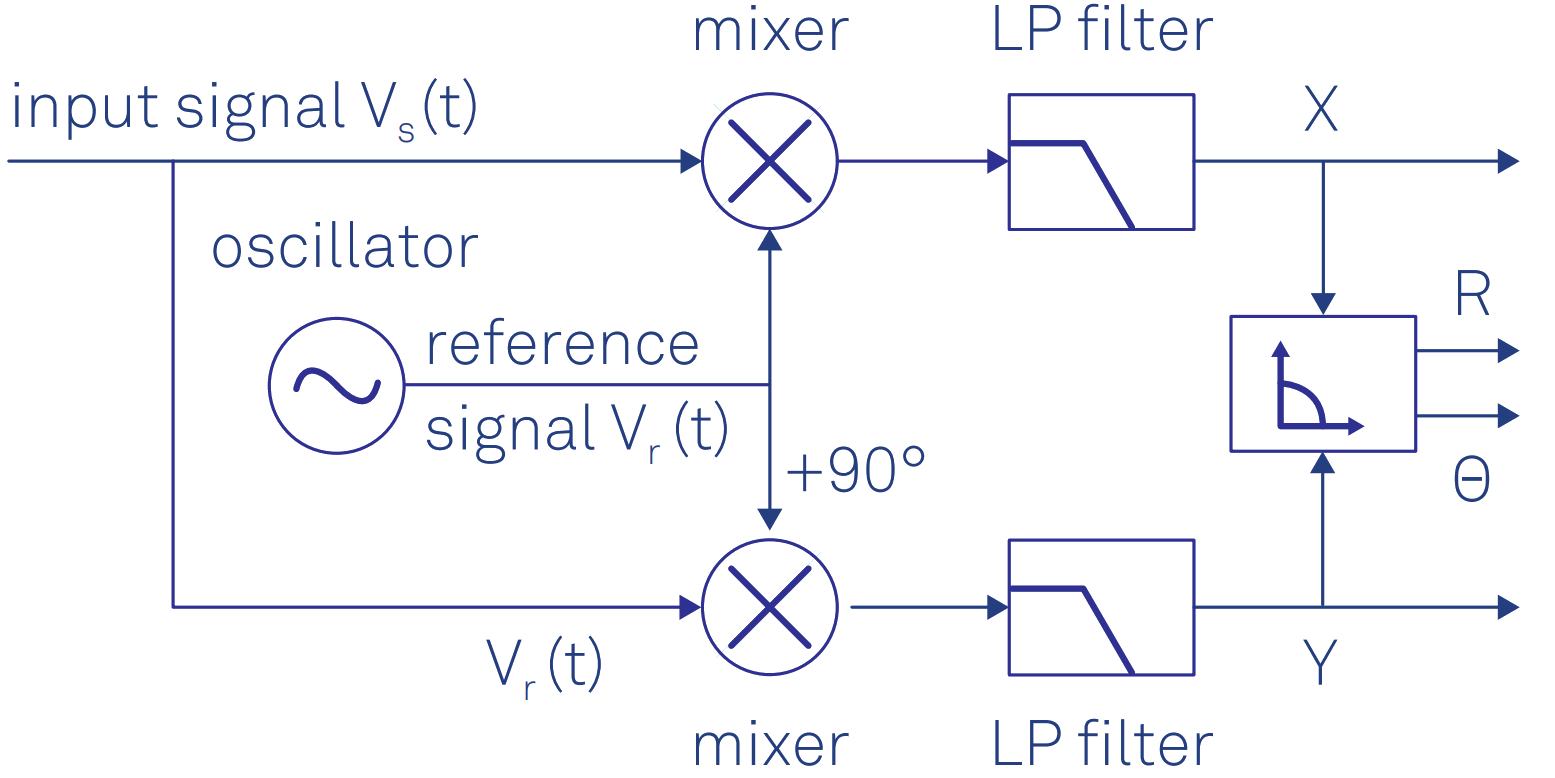
\includegraphics[width=0.7\linewidth]{img/lia_hl_schematic}
	\caption{High-level diagram of a \gls{lia} (image credit to Zurich Instruments \cite{instruments2018principles})}
	\label{fig:liahlschematic}
\end{figure}

Figure \ref{fig:liahlschematic} shows an overview of how lock-in amplification works. Simply put, the amplifier receives a signal $V_s$ and extracts the data at the frequency of a reference signal $V_r$. To explain this more thoroughly, lock-in amplification utilizes the fact that every signal is made of periodic waves, which are equal to zero when averaged. 

\begin{equation}\label{eq:voltage_sig}
	V_s = R\cos{(\omega_st + \theta)} = \frac{R}{2}e^{i(\omega_st + \theta)} + \frac{R}{2}e^{-i(\omega_st + \theta)}
\end{equation}

Equation \eqref{eq:voltage_sig} shows how the mathematical expression of a sine wave signal, where $\omega_s$ is the frequency and $\theta$ is the phase of the signal. Using the trigonometric identity $\cos{x} = \frac{1}{2}(e^{ix} + e^{-ix})$, the signal can be represented in terms of complex numbers.

\begin{equation}\label{eq:voltage_ref}
	V_r = e^{-i\omega_rt}
\end{equation}

In Equation \eqref{eq:voltage_ref}, a simplified reference signal is shown. Real applications might require more complex reference signals, but $V_r$ is perfect for demonstrating the lock-in principle.

\begin{equation}\label{eq:voltage_mult}
	V_m = V_sV_r = \frac{R}{2}e^{i(\omega_s -\omega_r)t  + \theta} + \frac{R}{2}e^{-i(\omega_s +\omega_r)t + \theta}
\end{equation}

Finally, Equation \eqref{eq:voltage_mult} shows the product of the signal $V_s$ and the reference $V_r$. In the case of $\omega_s = \omega_r$, there is a signal at \num{0} \unit{\hertz} and another one at $2\omega_s$ \unit{\hertz}. The latter, however, should be attenuated to an undetectable level by the low-pass filters shown in Figure \ref{fig:liahlschematic}. This way, both the unwanted signal appearing at double the frequency and all of the noise at different frequencies is attenuated.


